\chapter{Architecture}
\label{cha:architecture}

This chapter is dedicated to displaying and describing the numerous components,
their relationships, and the general needs for the cluster architecture's composition.
\\ %
Understanding how the cluster works lays a good foundation for the following chapters,
in which almost everything seen here is extensively explained in terms of how it
was developed and why certain decisions were taken. Furthermore, the design is
dynamic and may be modified to include more or fewer components and/or
requirements to better meet the requirements of the end user. \\ %
To prevent resource waste at the cost of a little decreased service interruption,
the overall design is structured around a high availability model rather than a fault
tolerance approach. Fault tolerance is based on specialized hardware that
detects a hardware fault and switches to a redundant hardware component
immediately. Although the transition seems to be seamless and provides continuous
service, a significant price is paid in terms of both power consumption and
performance since the redundant components do no processing but are constantly
operational. More crucially, the fault-tolerant paradigm ignores software errors,
which are by far the most prevalent cause of downtime. High availability, on the
other hand, considers availability to be a collection of system-wide, shared resources
that cooperate to ensure essential services, rather than a series of replicated
physical components. When a system, component, or application fails, high
availability combines software and hardware to minimize downtime by quickly
restoring essential services. While not instantaneous, services are generally
restored in less than a minute\cite{high_availability_vs_fault_tolerance}. \\ %
Section \ref{subsec:architecture_cluster_example} depicts a real-world functioning
example of the cluster design given. It has been extensively tested and is
continuously operational 24 hours a day, hosting a variety of services.
Furthermore, it upscales or downscales automatically dependent on demand or requirements.
\\ %
The diagram below illustrates the architecture, encompassing its components and
how they are interconnected, as well as a potential connection to an external network.

% TODO Full width
\begin{figure}[htbp]
  \centering
  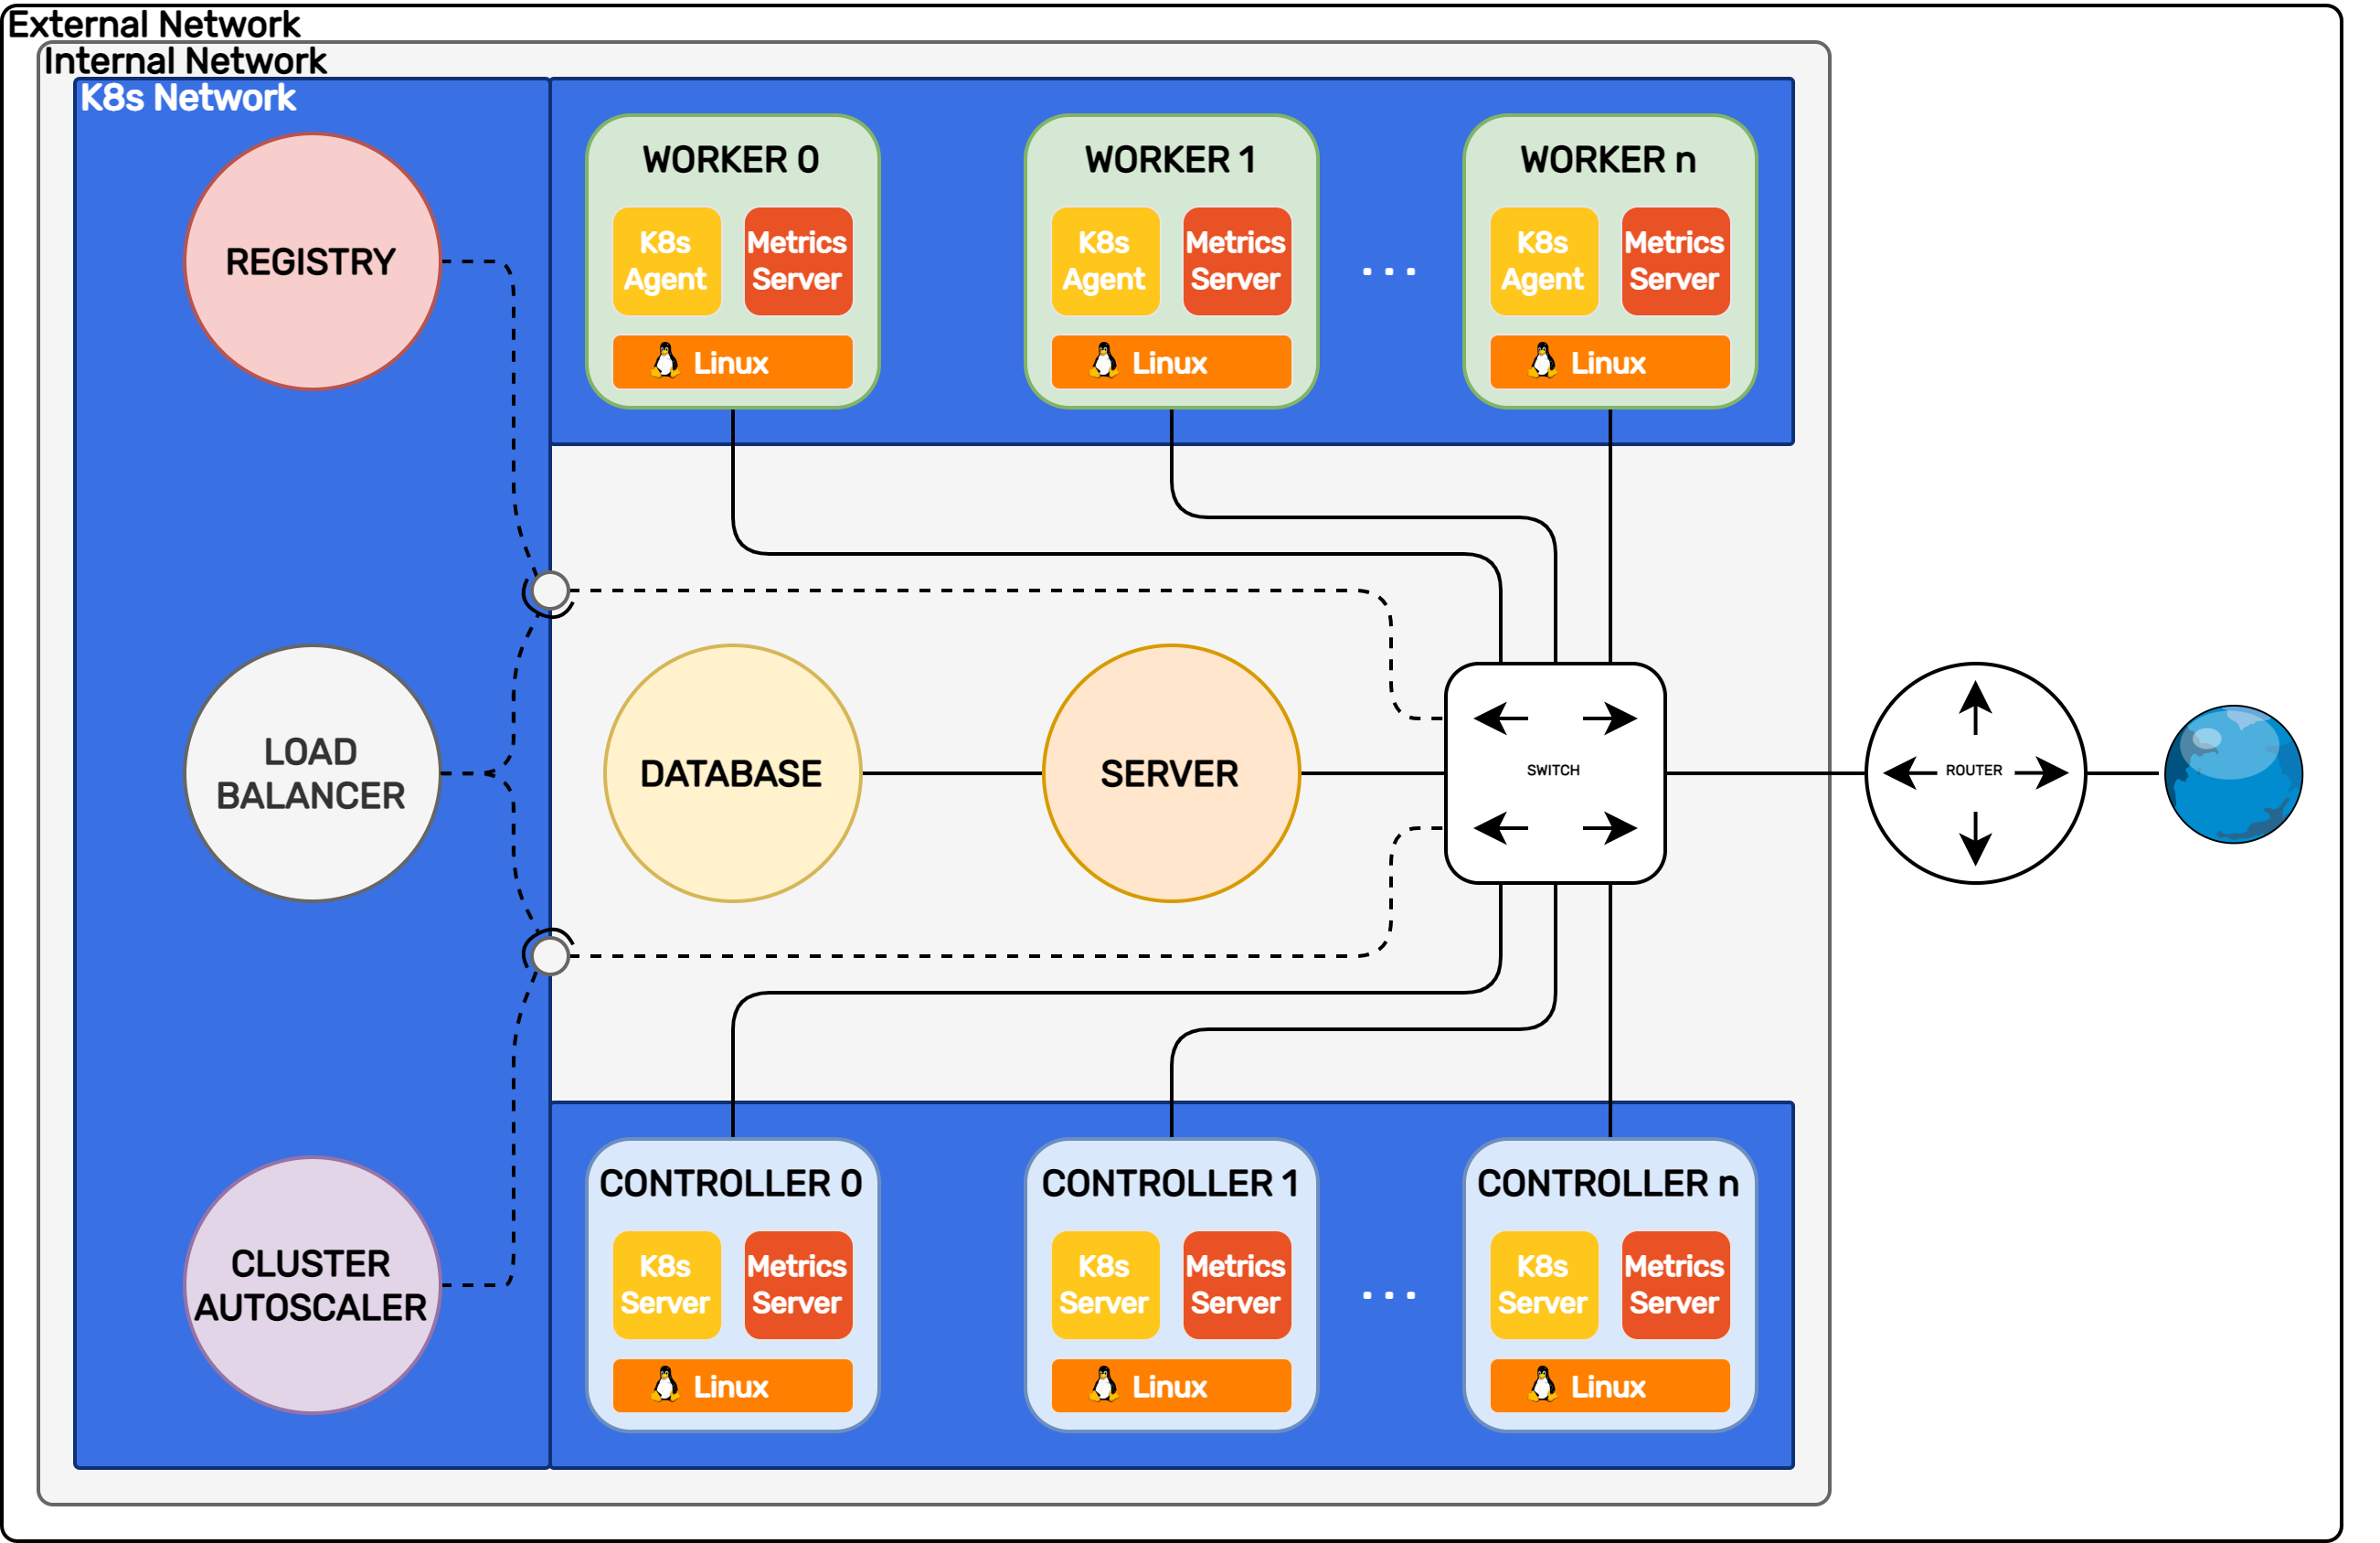
\includegraphics[width=.9\textwidth]{images/recluster/architecture.png}
  \caption{Architecture overview}
  \label{fig:architecture}
\end{figure}

\section{Components}
\label{sec:architecture_components}

\subsection{Node}
\label{subsec:architecture_components_node}

A node is a physical computer that runs the \texttt{Linux Kernel} and constantly
executes software that is specific to the cluster's composition. Linux is a
clone of the operating system Unix\footnote{\url{https://unix.org}}, written from
scratch by Linus Torvalds\footnote{\url{https://wikipedia.org/wiki/Linus_Torvalds}}
with help from a loosely-knit team of hackers across the world. It aims towards
POSIX and Single UNIX Specification compliance\cite{linux}.\\ %
Each node is physically connected to the other nodes via Ethernet and to the
many operating services/components through a virtual network. Section \ref{sec:architecture_network}
goes into further detail about cluster networking. \\ %
A node can be in one of two states. The \texttt{active} state indicates that a node
is turned on and is actively contributing to the cluster. The \texttt{inactive} state,
on the other hand, shows that a node has been turned off and is no longer actively
contributing to the cluster. This does not imply that the node is worthless and
will never be utilized again, but simply that it is no longer required for the current
cluster demand. A node state can be changed manually by switching the power
button on or off, or automatically through the Cluster Autoscaler component,
which monitors the current cluster state. More details about Cluster Autoscaler may
be found in section \ref{subsec:architecture_components_cluster_autoscaler}. \\ %
% TODO Maybe K8s reference section ?
Two core services are continuously operating on each node. The first service is
a Kubernetes-compliant distribution. Kubernetes, also known as K8s, is an open-source
solution for automating containerized application deployment, scaling, and administration\cite{k8s}.
The second service, Metrics Server, is a server that constantly monitors the node,
exposing hardware and operating system metrics. \\ %
Finally, each node is conceptually divided into two types depending on its role in
the cluster: Worker nodes and Controller nodes. These are discussed in the sections
that follow.

\subsubsection{Worker}
\label{subsubsec:architecture_components_node_worker}

\begin{wrapfigure}
  {l}{0pt} %
  \raisebox{0pt}[\dimexpr\height-\baselineskip\relax]{\centering
  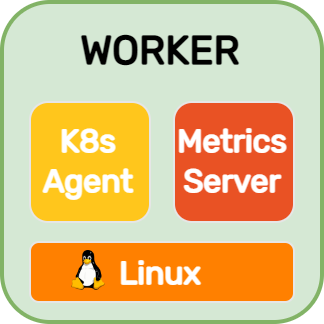
\includegraphics[width=.2\textwidth]{images/recluster/worker.png}}
\end{wrapfigure}

A worker node is designed to handle only deployable units of computation and services
that are not critical components of the cluster. It is not in charge of
scheduling the work over several nodes; rather, it only accepts it from a
cluster-available authenticated and authorized controller node. \\ %
Even though a worker node executes the effectively scheduled workload in the
cluster, it is not considered a critical component of it. At any given time, the
total number of active workers might be zero. That is, there is no scheduled workload,
and previously worker nodes have been shut down automatically to prevent
precious resource waste that is no longer required. \\ %
The majority of the cluster's accessible machines are worker nodes. This raises the
overall amount of schedulable workload as well as heterogeneity. Heterogeneity
is helpful because it may help schedule workloads to nodes with the bare minimum
of requested resources, preventing waste. Assume that the total number of
\texttt{active} nodes in the cluster is zero and that there are two \texttt{inactive}
worker nodes. The first node has 4 GiB of memory and consumes 100W of power,
whereas the second node has 8 GiB of memory and consumes 150W of power. A workload
using around 3GiB of memory is then planned for the cluster. Because it
decreases resource waste, notably memory waste, the first worker node will be
chosen. It is important to note that if both nodes have an equal amount of memory,
the conclusion remains the same since it has the lowest power consumption.

\subsubsection{Controller}
\label{subsubsec:architecture_components_node_controller}

\begin{wrapfigure}
  {l}{0pt} %
  \raisebox{0pt}[\dimexpr\height-\baselineskip\relax]{\centering
  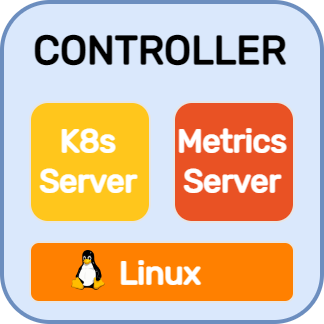
\includegraphics[width=.2\textwidth]{images/recluster/controller.png}}
\end{wrapfigure}

A controller node is an essential component of the cluster, acting as a coordinator
between the active worker nodes and the overall workload in the cluster. It
continually monitors the cluster's state in terms of available nodes, how and where
the workload should be scheduled, and much more. A consistent and secure API must
be provided for administration and end-users who wish to deploy custom services in
the cluster. The API can be made available to an external network if it is
available and appropriately configured, allowing remote control and improving overall
usage. \\ %
To ensure the integrity and management of a cluster, at least one controller
node must be constantly available. It is strongly suggested to have multiple controller
nodes that meet the high availability model to withstand potential system,
component, or application failures. This is possible considering an odd number
of controller nodes (i.e. three) that are always active. A quorum of controller
nodes is required for a cluster to agree on cluster state updates. Quorum in a cluster
with \texttt{n} controllers is \texttt{(n / 2) + 1}. Adding one node to any odd-sized
controller group will always increase the number of nodes required for a quorum.
Although adding a node to an odd-sized controller group appears to improve fault
tolerance since there are more machines, it worsens it because the same number
of nodes can crash without losing quorum but there are more nodes that can fail.
If the cluster cannot withstand any more failures, adding a node before removing
nodes is dangerous because if the new controller node fails to register, the cluster
quorum would be permanently lost\cite{quorum}. The latter is not a strict necessity,
but rather a preferable practice, even though it may slightly increase total resource
waste. Consider this: if the only available controller node encounters a software
or hardware failure and becomes unavailable, the entire cluster becomes
unreachable and unusable.\\ %
To further decrease overall resource waste, a controller can also become a
worker at the same time. If the overall workload in the cluster is very low and non-zero,
having one worker and one controller active with minimal utilization at the same
time is a waste. A single machine can perform the same task, saving precious
resources. If the entire demand grows later and the sole active node becomes overloaded,
the cluster reverts to its previous state. This is a configuration that may be enabled
or disabled based on the management needs of the cluster. \\ %
It should be noted that the total number of active or inactive nodes in the cluster
is not limited. However, a large number of nodes increases the workload on controller
nodes, which must maintain the cluster state updated and synchronized. As a result,
as shown in table \ref{tbl:controller_node_requirements}\cite{k3s_requirements},
their number and hardware requirements must be carefully balanced.

\begin{xltabular}
  {\textwidth} { c | >{\ttfamily}c | >{\ttfamily}c | >{\ttfamily}c }

  \multicolumn{1}{ c |}{\large{\textbf{Deployment Size}}} &
  \multicolumn{1}{ c |}{\large{\textbf{Nodes}}} &
  \multicolumn{1}{ c |}{\large{\textbf{CPU Cores}}} &
  \multicolumn{1}{ c}{\large{\textbf{RAM Memory}}} \\ \hline \hline

  Small & \raisebox{0.5ex}{\texttildelow}10 & 2 & 4 GiB \\ \hline

  Medium & \raisebox{0.5ex}{\texttildelow}100 & 4 & 8 GiB \\ \hline

  Large & \raisebox{0.5ex}{\texttildelow}250 & 8 & 16 GiB \\ \hline

  X-Large & \raisebox{0.5ex}{\texttildelow}500 & 16 & 32 GiB \\ \hline

  XX-Large & 500+ & 32 & 64 GiB \\

  \caption{Controller node requirements based on cluster size}
  \label{tbl:controller_node_requirements}
\end{xltabular}

\subsection{Server}
\label{subsec:architecture_components_server}

\begin{wrapfigure}
  {l}{0pt} %
  \raisebox{0pt}[\dimexpr\height-\baselineskip\relax]{\centering
  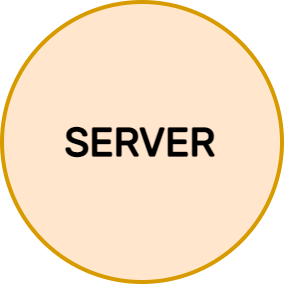
\includegraphics[width=.2\textwidth]{images/recluster/server.png}}
\end{wrapfigure}

A server handles all cluster nodes, user authentication and authorization, and much
more. It does not directly monitor the workload in the same way as a controller
node does, but it does serve as a low-level middleware controller. Every action
is made because of human intervention (e.g., administrators) or another
component of the cluster that has much higher-level knowledge of the current
state and reacts appropriately. \\ %
It is both an essential and a non-essential component of the cluster. It is essential
in the sense that it is aware of all registered nodes, both active and inactive,
and understands how to switch them on and off automatically. It reduces resource
waste by automatically increasing or decreasing the number of nodes in the
cluster when used in conjunction with the Cluster Autoscaler component (see section
\ref{subsec:architecture_components_cluster_autoscaler}). Without prior information,
there is no component in the cluster that can operate as an oracle about the
nodes, leaving the Cluster Autoscaler worthless and increasing total resource waste.
It is also deemed non-essential in the sense that, while decreasing resource waste
is the overall architecture's goal, there is no requirement for a high
availability model as in controller nodes. If a server instance crashes and does
not restart, leaving no more servers in the cluster, the entire cluster continues
to function normally. However, unless failures, human interaction, or server restarts,
the number of active nodes remains constant, potentially increasing resource waste.
\\ %
A server instance does not have to run on a dedicated node. A node can hold
numerous components at the same time, as previously mentioned. A node may be a
server, a controller, and a worker all at the same time, drastically decreasing resource
waste. It is crucial to note, however, that a server should not be executed on a
worker node since, as previously explained, the total number of active workers
might be zero, terminating the server instance and the capability of automatically
adjusting the cluster size. \\ %
The server provides an API to facilitate cluster administration. Furthermore, as
previously said, it is in charge of user authentication and authorization. Unharmful
queries (providing information about active nodes or listing non-sensible
information about a user) should not require any authentication or only a minimal
one. Queries that mutate the state of the cluster or display sensitive
information (turning on or off a node or displaying sensitive user information)
must be protected by a high-security mechanism. \\ %
A heartbeat daemon must be implemented on the server to continuously check the
condition of a node and detect any problems. A heartbeat is a periodic signal or
message created by hardware or software that is sent between devices at regular intervals
of seconds. If the endpoint does not receive a heartbeat for an extended period,
often many heartbeat intervals, the machine that should have sent the heartbeat
is assumed to have failed\cite{heartbeat}. The latter is commonly implemented by
controller nodes since they must constantly monitor and acquire information
about active nodes for workload scheduling. As a result, a server can use the
controller's API to eliminate duplication, increase consistency and availability,
and simplify implementation. \\ %
For more information, section \ref{sec:implementation_server} covers in detail how
the server component is implemented.

\subsection{Database}
\label{subsec:architecture_components_server_database}

\begin{wrapfigure}
  {l}{0pt} %
  \raisebox{0pt}[\dimexpr\height-\baselineskip\relax]{\centering
  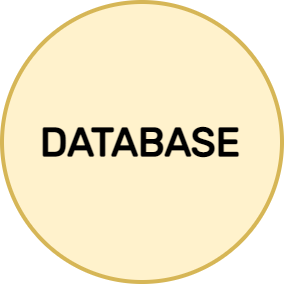
\includegraphics[width=.2\textwidth]{images/recluster/database.png}}
\end{wrapfigure}

The database component is strictly related to the server component. Its primary
function is to store all cluster-related data in a safe, persistent and fault-tolerant
system. The data in question is generally static and does not change frequently.
Static data includes all node-related information, such as CPU type and RAM
quantity, that is hardly modified after the node is added to the cluster.
However, some data, like information regarding the current node state and its
last heartbeat, are intrinsically dynamic in the sense that the system regularly
changes them to ensure integrity. Like the server component, is seen as both necessary
and non-essential. A server is worthless without the database, resulting in the same
outcome as previously explained. \\ %
This component is seen as the union of numerous modules that form it rather than
as a single entity. A database, in general, is a structured collection of
information or data that is persistently stored in a computer system. A database
management system (DBMS) is a software program that acts as an interface between
the database and its end users or applications, allowing for the retrieval, updating,
and administration of how information is structured and optimized. A DBMS also facilitates
database supervision and control by providing several administrative operations such
as performance monitoring, tuning, and backup and recovery\cite{database}. The latter
indicates that each module and feature is dependent on the implementation. Only
for the database itself, there are several distinct types, and for each type, there
are numerous distributions with varying features and capabilities. To better
follow the overall design criteria, the ultimate decision on which one to take must
be carefully examined. \\ %
Persistency and fault tolerance are strongly related, most importantly, in the data
layer. Even if an error occurs, the only vital and critical component that must be
preserved and not lost is all the stored data. Data persistency is the
preservation of data after the program that produced it has been terminated. To do
this, the data must be written to non-volatile storage, a type of memory that can
maintain the information indefinitely even if the program is no longer functioning\cite{persistency}.
Fault tolerance, which differs slightly from the previous definition, refers to a
non-volatile storage system's capacity to recover from an error or faulty condition,
most typically an irreversible hardware failure of some type, without losing any
previously stored data. Disk fault tolerance is often achieved by disk
management technologies such as mirroring\footnote{\url{https://wikipedia.org/wiki/Disk_mirroring}},
data striping\footnote{\url{https://wikipedia.org/wiki/Data_striping}},
duplexing\footnote{\url{https://www.pcmag.com/encyclopedia/term/disk-duplexing}},
and Redundant Array of Independent (or Inexpensive) Disks (RAID)\footnote{\url{https://wikipedia.org/wiki/RAID}}\cite{disk_management_technologies}.
Consider the possibility that the database component has a hardware failure and ceases
to operate. The damage has compromised not just the replaceable hardware (such as
the CPU, motherboard, and RAM), but also some (but not all) storage devices storing
the cluster's data. Typically, all data is irreversibly lost, and the cluster
must be rebuilt from scratch. However, with a correctly designed disk management
system, once the faulty hardware is replaced, all data is automatically
recovered and the cluster becomes functional again. The process of rebuilding the
data might take a significant amount of time (i.e. calculating the parity bit\footnote{\url{https://wikipedia.org/wiki/Parity_bit}}).
\\ %
Finally, an optional cache middleware can be implemented between the server and database,
enhancing read speed for frequently requested but rarely updated data and
reducing disk utilization. The cached data is stored in the main volatile memory.

\subsection{Registry}
\label{subsec:architecture_components_registry}

\begin{wrapfigure}
  {l}{0pt} %
  \raisebox{0pt}[\dimexpr\height-\baselineskip\relax]{\centering
  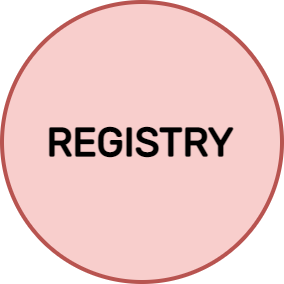
\includegraphics[width=.2\textwidth]{images/recluster/registry.png}}
\end{wrapfigure}

% TODO Air-Gap reference
% TODO Container reference

The registry component is a private container registry that the K8s orchestrator
uses in the cluster to download a specific image or collection of images. A container
registry is a stateless, highly scalable server-side application that stores and
distributes container-based application images\cite{container_registry}. \\ %
A registry is regarded as a non-essential component because the whole system may
function without it. If an internet connection is available and one of the
numerous public container registries (such as Docker Hub\footnote{\url{https://hub.docker.com}})
is accessible, the cluster downloads and runs the requested image from the external
network. Having a private register in the cluster, on the other hand, may solve
a plethora of potential difficulties. Some of them are as follows:

\begin{itemize}
  \item The K8s orchestrator fails to download the requested images in an Air-Gapped
    environment when there is no internet connection. As a result, the entire cluster
    is nearly unusable. The only realistic approach is to make a local duplicate
    of the remote images for each cluster node. This is hard to accomplish and prone
    to errors. Furthermore, there is a waste of disk memory, but it also ignores
    how and where the images are downloaded.

  \item A local solution is required for an organization that wants complete control
    over its images and is unwilling to put them on an external service.
    Furthermore, if the organization takes a security-first approach, a properly
    configured private registry can improve overall security.

  \item A newly developed image that must be evaluated before beginning release to
    production. Moreover, the registry may be used to improve DevOps techniques by
    preventing potential bugs, security vulnerabilities, and other difficulties that
    can arise in a real-world environment. Attachment \ref{cha:good_practices}
    goes into much depth about DevOps.

  \item An image created exclusively for the cluster. Uploading it to a public
    registry is not only pointless due to incompatibility, but it also limits the
    available namespace because an image name must be unique.

  \item Registry as a pull-through cache\footnote{\url{https://docs.docker.com/registry/recipes/mirror}}.
    If multiple cluster nodes require the same external image and it does not
    exist locally, each of them fetches it from the specified registry. This
    results in excessive and inefficient network utilization, which might congest
    the cluster. The private registry can act as a registry mirror, locally caching
    each externally requested image. Every node points directly to the private
    registry address. If an image cannot be located locally, the request is
    routed to the local registry, which downloads and caches it. When a node
    requests the same image again, the registry provides the cached image without
    needing any further network traffic.
\end{itemize}

In practice, the registry is used to distribute the Cluster Autoscaler image (see
\ref{subsec:architecture_components_cluster_autoscaler}) that is specifically built
to function with reCluster. \\ %
Even though it is supported out of the box, the component does not need to be
instantiated on a specific physical node; rather, it is deployed directly in the
K8s environment. The registry may be accessible from both inside and outside the
K8s network, thanks to a correctly configured Load Balancer component (further information
in section \ref{subsec:architecture_components_load_balancer}) that exposes the
service to a non-K8s-related external network. Exposing the K8s service is critical
for conveniently allowing the upload (push) and download (pull) of an image without
the user requiring any extra settings. The approach must remain the same as when
utilizing a publicly accessible registry, but with the cluster's registry address
provided. Because the registry is externally accessible, it must be properly configured
to improve overall security. HTTPS\footnote{\url{https://wikipedia.org/wiki/HTTPS}},
which enables secure communication over a cryptographic channel, and
authentication, which permits access only to a limited group of authenticated users,
must be set up and/or implemented. \\ %
The registry is deployed in the K8s environment, but the K8s orchestrator needs it
to fetch the required images, leading to a circular dependence. To avoid the latter,
the registry image should be made available on each node, eliminating the need for
a registry request.

\subsection{Cluster Autoscaler}
\label{subsec:architecture_components_cluster_autoscaler}

\begin{wrapfigure}
  {l}{0pt} %
  \raisebox{0pt}[\dimexpr\height-\baselineskip\relax]{\centering
  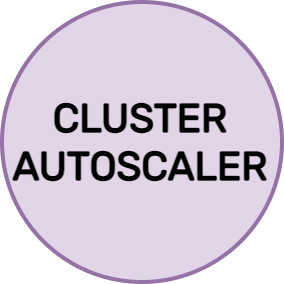
\includegraphics[width=.2\textwidth]{images/recluster/cluster_autoscaler.png}}
\end{wrapfigure}

% TODO K8s reference

The Cluster Autoscaler component is a program that automatically adjusts the
number of nodes in the cluster to guarantee that all deployed services have a
location to execute and no nodes are underutilized\cite{cluster_autoscaler}. It
is not in charge of node behavior and registration in the cluster; it only determines
if a node should be turned on or off, but not how. As a result, for low-level
control, it must rely on the server component. Nonetheless, the autoscaler is an
essential component of the cluster due to its automation, which eliminates the
need for human interaction and dramatically lowers resource waste. \\ %
The Cluster Autoscaler is deployed in the K8s environment rather than on a
separate node. After the registry becomes available, the container image of the
autoscaler is uploaded and made available to the whole cluster during the
initialization phase. Because the registry is defined as a critical K8s service,
it may be scheduled on any node, both workers and controllers. Since the cluster
may scale to zero workers, this applies to every critical component in the K8s environment,
preventing a service outage. Furthermore, the cluster autoscaler must be
maintained operational at all times: if a crash or error happens, it must be
restarted. The latter is accomplished automatically by the K8s system, removing
the need for a custom solution. \\ %
The component has both a high-level and a low-level view of the cluster. The high-level
view is accomplished by continuously monitoring the cluster's condition to ensure
its integrity: workload and active nodes. As a result, it is aware of whether
there are services that cannot be deployed owing to a lack of resources, or if there
are underutilized active nodes for the present demand, resulting in resource
waste. This is accomplished by directly querying the protected API provided by the
controller nodes. Far from it, the low-level view is obtained by continually updating
a local cache that contains all of the available nodes in the cluster, both
active and inactive, to know how many nodes are available and their status. As a
result, it is aware of the nodes that can be turned on or off, as well as if the
system can be scaled up or down. As previously stated, the latter is
accomplished by accessing the server on a series of secured API endpoints that
provide direct control over how the cluster's nodes are handled. \\ %
The prerequisites and solutions for automatically adjusting the cluster size are
outlined below:
\begin{itemize}
  \item There are some computing units (pods) that are unable to operate in the cluster
    owing to a lack of resources.
    \newline
    If the cluster's current total workload with the present number of active
    nodes has reached its maximum, it will be unable to support further service deployments.
    This indicates that newly deployed services are never executed and are
    always in a state of waiting. In this condition, the controllers continue to
    monitor the cluster's condition for a suitable node with enough free
    resources to host a waiting service. Waiting forever for a current active node
    to free up some resources affects the cluster's overall usability and quality
    of service\footnote{\url{https://wikipedia.org/wiki/Quality_of_service}} (QoS).
    The solution is to check if there is a suitable inactive node in the local
    cache that can be turned on. If such a node is identified, a specific
    request is issued to the server, and the queued deployments are automatically
    scheduled to the newly bootstrapped node.

  \item Some nodes are constantly unneeded for an extended period. When a node's
    resource utilization is low and all of its scheduled deployments can be
    transferred to another node, it is no longer required.
    \newline
    There is a waste of resources if the current workload on a node falls below
    a pre-defined threshold for a certain period. To avoid this, all deployments
    on the node must be rescheduled to another node with sufficient free
    resources, raising its overall utilization. Following completion of the
    latter, the unneeded node has almost zero workloads (non-zero since there
    may be system deployments running that do not require a migration and may be
    deleted) and can be switched off and removed. The autoscaler makes a
    specific request to the server with the node identifier; the server removes the
    node from the K8s environment and subsequently shuts it off altogether. When
    a node is successfully shut down, its status changes from active to inactive,
    indicating that it is a candidate for an eventual upscaling.
\end{itemize}

\subsection{Load Balancer}
\label{subsec:architecture_components_load_balancer}

\begin{wrapfigure}
  {l}{0pt} %
  \raisebox{0pt}[\dimexpr\height-\baselineskip\relax]{\centering
  
\includegraphics[width=.2\textwidth]{images/recluster/load_balancer.png}}
\end{wrapfigure}

% K8s reference
The load balancer component provides an externally accessible IP address to an
internal K8s application. It may be seen as an abstract mechanism of exposing the
application as a network service without requiring an unfamiliar service discovery
mechanism\cite{load_balancer}. \\ %
An application can be composed of multiple replicas that are generated and
destroyed to maintain the cluster in the desired state. The replicas can be spread
over many active nodes, improving overall performance, availability, and fault
tolerance. When an application is created in a K8s environment, there is no way
to connect from outside the cluster by default. As a result, only other K8s
deployments can communicate with it. A load balancer acts as a solution by routing
external network traffic to the cluster node where a replica of the application is
deployed. To prevent scenarios where some replicas are overloaded and others are
not, it does allow different network traffic policies (such as Round-robin\footnote{\url{https://wikipedia.org/wiki/Round-robin_item_allocation}},
random, and others) to homogeneously distribute traffic across all replicas. As
a result, it serves as a consistent and fixed entry point for connecting to the potentially
numerous application replicas that are intrinsically dynamic due to their non-permanent
resources (i.e., internal IP address). \\ %
At first, considering the architecture schema, it is unclear if it is an essential
or non-essential component. Its utilization, however, is tightly associated with
the kind and usage of deployed applications/components in the cluster. For example,
if the cluster is intended to host numerous web applications that must be
accessed over the internet, a load balancer component is necessary to expose each
application to external network traffic. If the cluster is just used for testing
or DevOps techniques (see attachment \ref{cha:good_practices}), there is no need
to expose any applications, leaving the load balancer components unnecessary. As
a result, it can be removed, increasing the total available resources. \\ %
In data centers operated by huge cloud providers like Microsoft\footnote{\url{https://azure.microsoft.com}},
Google\footnote{\url{https://cloud.google.com}}, or Amazon\footnote{\url{https://aws.amazon.com}},
a load balancer is generally an external, sophisticated, and highly specialized
component that is specifically designed to be compatible with the specific cloud
provider. The general architecture in question, however, is far simpler and operates
on bare-metal servers. A bare-metal server is a physical computer that is
exclusively operated by one customer or tenant\cite{bare_metal_server}. As a
result, an external load balancer may be substituted with an internal one that is
deployed directly in the K8s environment. An internal load balancer minimizes
overall resource usage while also improving maintainability. Furthermore, as
with the registry and cluster autoscaler components, the internal load balancer is
kept automatically operational and in good working condition at all times by the
K8s orchestrator.

\subsubsection{Example Schema}
\label{subsubsec:architecture_components_load_balancer_schema}

Figure \ref{fig:load_balancer} depicts an example schema of an Internal Load
Balancer in a cluster architecture. It is worth noting that the Internal Load Balancer
component is presented externally to the nodes to simplify the overall overview but
in reality, it is deployed directly on each active node.

\begin{figure}[htbp]
  \centering
  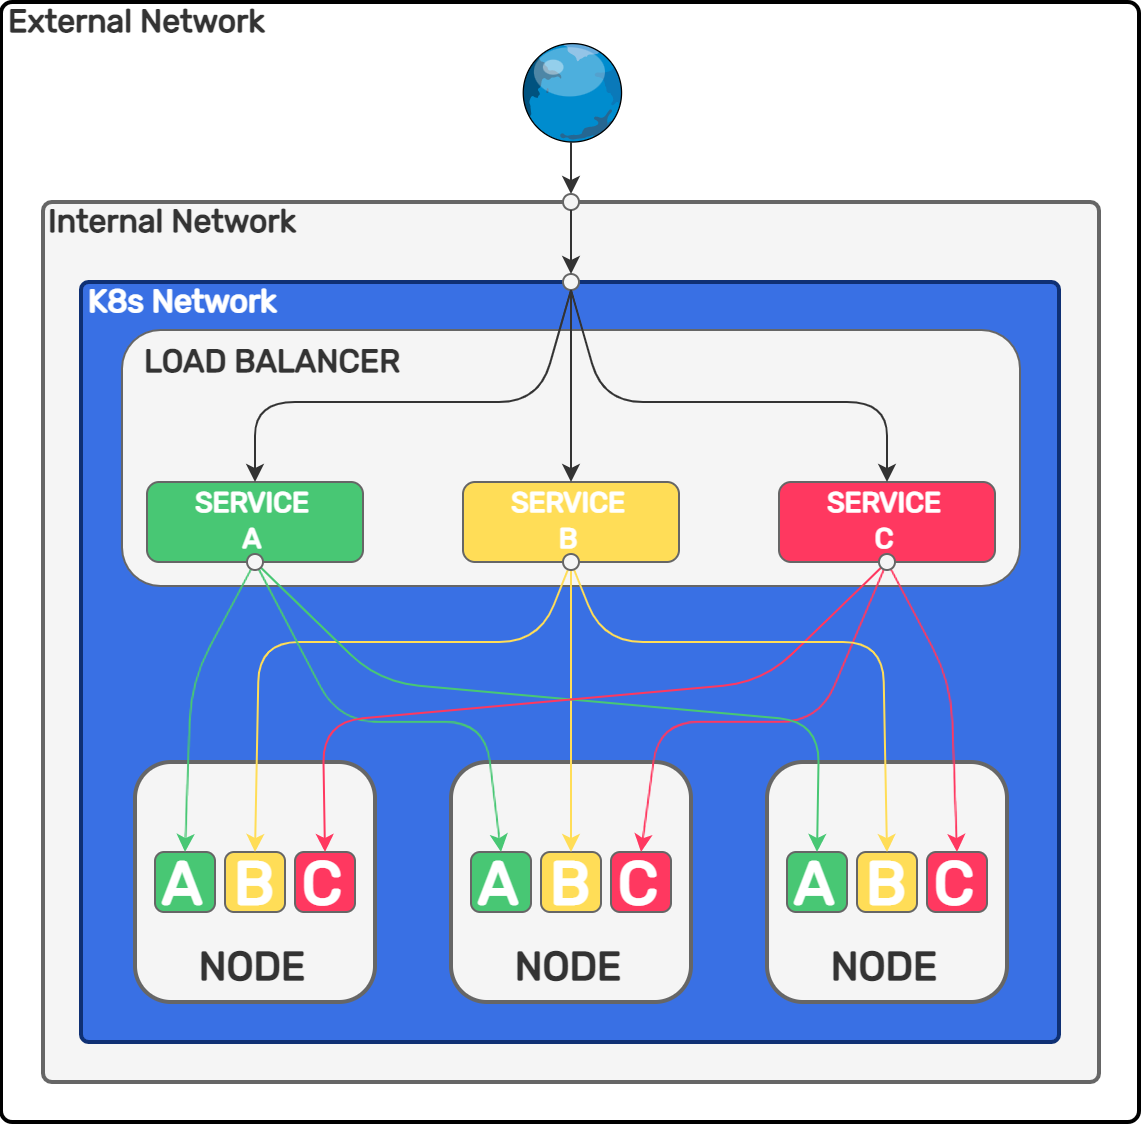
\includegraphics
  [width=.7\textwidth]{images/recluster/load_balancer_example.png}
  \caption{Internal Load Balancer schema example}
  \label{fig:load_balancer}
\end{figure}

There are three active nodes and one Internal Load Balancer in the cluster. The
nodes' roles have not been specified, however as stated in section
\ref{subsec:architecture_components_node}, each node can be regarded as both a Controller
and a Worker. Three applications, \texttt{A}, \texttt{B}, and \texttt{C}, have been
deployed in the K8s environment, with three replicas available for each. Concerning
the other replicas, each replica is scheduled on a distinct node. \\ %
The organization in charge of the cluster wishes to expose each application by
assigning each one a unique externally accessible IP address from the Internal
Network (i.e., a private IPv4 address\footnote{\url{https://wikipedia.org/wiki/Private_network}}).
It should be noted that the process of mapping/routing an IP address from the Internal
Network to an IP address from the External Network is not mentioned. The Load
Balancer creates a matching internal service for each application that knows
where all the replicas are installed and how to efficiently distribute traffic
among them. Assume that application \texttt{A} is assigned the IP address
\texttt{10.0.0.97} and that the Load Balancer receives an external request from a
client on the Internal Network. The Load Balancer examines the target address
and finds a match; the request is then routed to internal service \texttt{A}. Service
\texttt{A} then redirects the request to one of the active nodes where a replica
of application \texttt{A} is deployed. Finally, the replica handles the request,
and a response is created and sent back to the client.

\section{Network}
\label{sec:architecture_network}

The cluster is composed of several network layers, each of which may interact
with components of the same layer but by default, not with components of a different
layer. Each network layer is heterogeneous: various software/hardware components
and applications correlate to different network layers. The cluster can support
communications across layers, but this must be done transparently and accurately
to avoid significantly increasing the cluster's complexity and resource waste while
lowering its overall security. Both software and hardware components that reside
between the two communicating levels enable inter-layer communication. The most fundamental
requirement for the latter to work is that there be no potential conflicts between
the two communicating layers. \\ %
There are three distinct network layers in the cluster architecture seen in figure
\ref{fig:architecture}. They are covered in the subsections that follow, beginning
with the most external network and progressing to the most internal network in relation
to the cluster.

\subsection{External Network}
\label{subsec:architecture_network_external_network}

\begin{wrapfigure}
  {l}{0pt} %
  \raisebox{0pt}[\dimexpr\height-\baselineskip\relax]{\centering
  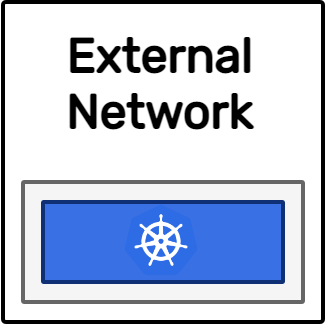
\includegraphics[width=.2\textwidth]{images/recluster/external_network.png}}
\end{wrapfigure}

The external network is any network that does not involves the cluster with direct
communications. It represents any network that is not compatible with the
Internal Network (see section below) and needs a router or other similar
components to allow the communication between the two. A router is a device that
connects two or more packet-switched networks or subnetworks. It serves two
primary functions: managing traffic between these networks by forwarding data packets
to their intended IP addresses, and allowing multiple devices to use the same
Internet connection\cite{https://www.cloudflare.com/learning/network-layer/what-is-a-router}.

To simplify, the external network can be seen as any existing network in the
world except the Internal Network, hence the Internet: the network of networks.

Access to the external network is necessiry if the deployed applications can be
accessed by external clients and there are the needs of external resources, such
as public container images, that are not locally available in the cluster. Moreover,
if the organization managing the overall architecture wants to have remote
control and monitoring of the cluster across the globe the only current viable
and supported solution is through an internet connection. If the latter are not needed,
the external network can be removed from the cluster architecture implying an
Air-Gap environment without internet connection. Hence, all needed resources and
components are already locally available and access to the cluster is only
needed from within the internal network.

An external network is intrinsecally unsecure. Therefore, high security
protocols, mechanisms and procedures must be implemented and correctly configured.
This is a very complicated topic that is not covered.

\subsection{Internal Network}
\label{subsec:architecture_network_internal_network}

\begin{wrapfigure}
  {l}{0pt} %
  \raisebox{0pt}[\dimexpr\height-\baselineskip\relax]{\centering
  
\includegraphics[width=.2\textwidth]{images/recluster/internal_network.png}}
\end{wrapfigure}

% Domain

\subsection{K8s Network}
\label{subsec:architecture_network_k8s_network}

\begin{wrapfigure}
  {l}{0pt} %
  \raisebox{0pt}[\dimexpr\height-\baselineskip\relax]{\centering
  
\includegraphics[width=.2\textwidth]{images/recluster/k8s_network.png}}
\end{wrapfigure}

% Overlay Network

\section{Cluster}
\label{sec:architecture_cluster}

\begin{wrapfigure}
  {r}{.5\textwidth}
  \centering
  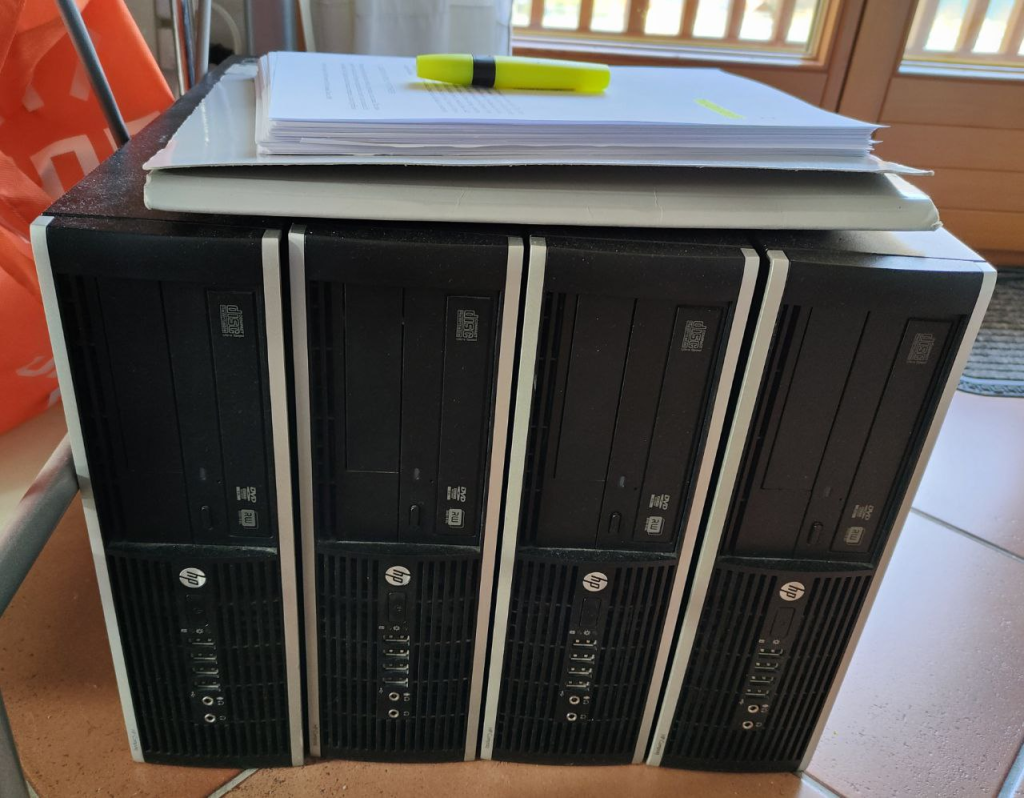
\includegraphics[width=.5\textwidth]{images/recluster/cluster.png}
  \caption{reCluster cluster}
\end{wrapfigure}

\subsection{Hardware}
\label{subsec:architecture_cluster_hardware}

% TODO WoL features, how to turn on nodes
% TODO Prefer nodes with WoL upscaling

\subsection{Example}
\label{subsec:architecture_cluster_example}

% TODO Move